\documentclass[conference]{IEEEtran}
\IEEEoverridecommandlockouts
% The preceding line is only needed to identify funding in the first footnote. If that is unneeded, please comment it out.
\usepackage{cite}
\usepackage{amsmath,amssymb,amsfonts}
\usepackage{algorithmic}
\usepackage{graphicx}
\usepackage{textcomp}
\usepackage{xcolor}
\def\BibTeX{{\rm B\kern-.05em{\sc i\kern-.025em b}\kern-.08em
    T\kern-.1667em\lower.7ex\hbox{E}\kern-.125emX}}
\begin{document}

\title{Designing a Minimum Distance to Class Mean Classifier\\
}

\author{\IEEEauthorblockN{Devopriya Tirtho}
\IEEEauthorblockN{16.02.04.033}
\IEEEauthorblockA{\textit{Department of Computer Science and Engineering} \\
\textit{Ahsanullah University of Science and Technology}\\
Dhaka, Bangladesh \\
}

}

\maketitle

\begin{abstract}
The field of study named \textbf{‘Machine Learning’} tends to learn from appropriate datasets and tries to interpret results from that learning. Classification is a part of Machine Learning which tries to use those Machine Learning algorithms which learn from ‘Train Data’ to find the accurate class for ‘Test Data’. \textbf{‘Minimum Distance to Class Mean Classifier’} is one of the forms of Classification Technique which is very accurate for predicting appropriate class with the help linear discriminant function.

\end{abstract}

\begin{IEEEkeywords}
Machine Learning, Classification, Algorithm, Dataset.
\end{IEEEkeywords}

\section{Introduction}
\textbf{‘Minimum Distance to Class Mean Classifier’} is a classification technique which trains itself with the training vectors to fix the classified mean point and based on that classified mean point calculates the appropriate class of unclassified vectors of more than one class. Training dataset suggests that there are ‘n’ number of classified samples with proper features’ values. With the help of a \textbf{‘Linear Discriminant Function’} and some basic criterions unknown vectors are classified. So, this method works on finding the appropriate class of unknown sample of vector where classes are of more than one class.


\section{Task}

There are two datasets named ‘train’ and ‘test’. From the ‘train’ dataset we can find the sample prototypes of two classes which are classified by number ‘1’ and ‘2’. Here are the datapoints of ‘train’ Dataset:\\
	W1= \{(2, 2), (3, 1), (3, 3), (-1, -3), (4, 2), (-2, -2)\}\\
	W2= \{(-4, 3), (2, 6), (0, 0), (-2, 2), (-1, -1), (-4, 2)\}\\
\begin{itemize}  
\item Firstly, we have to plot all the data points of each class with corresponding marker in graph.\\
  \item After plotting, we have to find the mean value of \textbf{‘Class 1’s’} points and \textbf{‘Class 2’s’} points.\\
  \item With the help of the following discriminant function we have to specify the appropriate class of the ‘test’ dataset.\\
 			 
  \item We have to draw the decision boundary to visualize the boundary of classification.\\
  \item Finally, we have to find the accuracy of the model for our given ‘test’ dataset.\\
\end{itemize}

\section{Experimental Design}
\begin{itemize}  
	\item \textbf{Plotting All Training Points:}
	In our given dataset which is named as ‘train’, we need to pick the values which represent X-coordinate values and Y-coordinate values. Then with appropriate marker and distinct color we have to plot the points of \textbf{‘Class 1’} and \textbf{‘Class 2’}.\\
	\item \textbf{Calculate the Mean Point:}
Then we have to find the mean point of \textbf{‘Class 1’} and \textbf{‘Class 2}’ by taking the mean of appropriate vectors and plot the mean points of ‘Class 1’ and ‘Class 2’ with appropriate marker in the graph.\\
	\item \textbf{Classify the Test Data:}
After finding the mean vectors of \textbf{‘Class 1’} and \textbf{‘Class 2’} we take the discriminant function for two classes as g1 and g2.\\
 Here,\\
$
g_1 (x)=w_1^T x-1/2 w_1^T w_1\\$

$
g_2 (x)=w_2^T x-1/2 w_2^T w_2\\$

By doing appropriate calculation for each data points of ‘test’ dataset we compare the values of g1 and g2 to find the appropriate class of each data point.
\begin{figure}[htbp]
\centerline{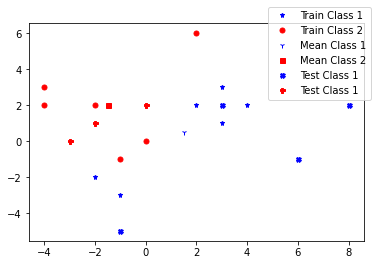
\includegraphics[width=8cm, height=4cm]{points.png}}
\caption{After classification of all testing points}
\label{fig}
\end{figure}

\item \textbf{ Drawing Decision Boundary:}
To distinguish the area of each class we need to draw the decision boundary. The mathematical form the decision boundary is given below:\\

	$g_1 (x)=g_2 (x)\\$

$
>w_1^T x-w_2^T x-1/2 (w_1^T w_1-1/2 w_2^T)=0\\$


$
>(w_1^T-w_2^T)x-1/2 (w_1^T w_1-1/2 w_2^T)=0\\$


$
>\begin{pmatrix}COEF_1  & COEF_2\end{pmatrix}
\begin{pmatrix} x_1\\x_2 \end{pmatrix}+CONSTANT=0\\$

Here,\\

$
CONSTANT=-1/2 (w_1^T w_1-1/2 w_2^T)\\$


$
>
(COEF_1×x_1+COEF_2×x_2 )+CONSTANT=0\\$

$
>x_2=(COEF_1×x_1+CONSTANT)/-COEF_2 \\$

By taking equidistance values for x1 for X-coordinate, we get the values for x2 for Y-Coordinate and plot the decision boundary with corresponding (x1, x2) point.\\

\begin{figure}[htbp]
\centerline{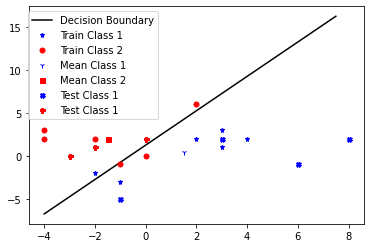
\includegraphics[width=8cm, height=12cm]{fr.png}}
\caption{Drawing of decision boundary}
\label{fig}
\end{figure}
\end{itemize}


\section{Python Code}
\begin{figure}[htbp]
\centerline{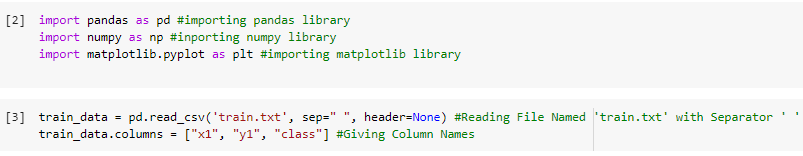
\includegraphics[width=8cm, height=4cm]{1.png}}
\centerline{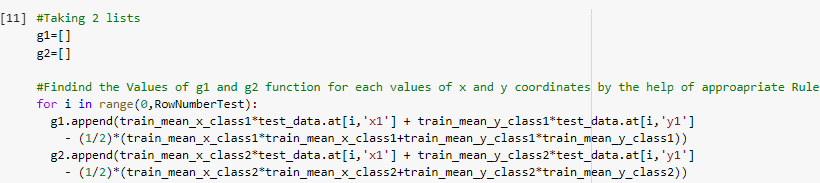
\includegraphics[width=8cm, height=4cm]{3.png}}
\centerline{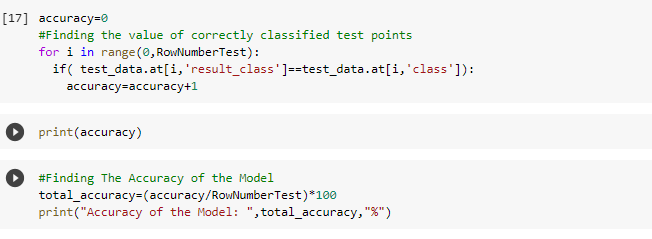
\includegraphics[width=8cm, height=4cm]{5.png}}
\centerline{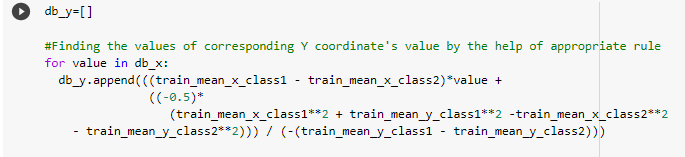
\includegraphics[width=8cm, height=4cm]{7.png}}
\centerline{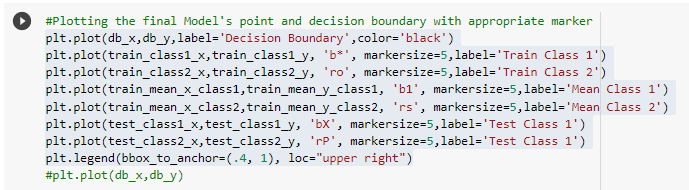
\includegraphics[width=8cm, height=4cm]{6.png}}
\caption{Snapshot of python code}
\label{fig}
\end{figure}

\section{Result Analysis}
The implemented model gives us the accuracy of \textbf{85.714\%} for the ‘test’ data where some of the results were misclassified.



\section{Conclusion}

\textbf{‘Minimum Distance to Class Mean Classifier’} is a simple classification technique which uses linear discriminant function to classify unknown classes. This model is not perfectly accurate as it gives us some misclassified result. Further improvement can be done using non-linear decision boundary to classify all the unknown data perfectly.




\end{document}
